\documentclass[12pt, draftclsnofoot, onecolumn]{IEEEtran}
%\documentclass[a4paper,12pt]{article}
\usepackage[english]{babel}
\usepackage[utf8]{inputenc}
\usepackage{amsmath}
\usepackage{graphicx}
\usepackage{subfigure}
\usepackage{xfrac}
\usepackage{color}
\usepackage{listings}
%\usepackage{slashbox}
\usepackage{indentfirst} 
\usepackage{cite}

%\usepackage[left=2cm, right=2cm, top=2cm, bottom=2cm]{geometry}

%\captionsetup[figure]{labelfont={small,rm,bf},labelsep=period,font={small,rm}}
\title{Wireless Communications Final Project \\COST 207 Channel Emulator}
\author{Name: Chia-Yu Liu, ID: 103064510}
\date{	}

\begin{document}
\maketitle
\section{Objectives and Methods}
In this project, we want to implement the \textit{COST 207} channel emulator, where there are four kinds of Doppler spectrums with different scattering functions. The first one is the classical Doppler spectrum (CLASS), where the Doppler scattering is assumed to be isotropic scattering. The second and third one are the Gaussian 1 Doppler spectrum (GAUS1) and the Gaussian 2 Doppler spectrum (GAUS2), respectively, which are non-isotropic scattering. The last one is the RICE Doppler spectrum that is isotropic scattering with line-of-sight propagation. In addition, there are several channel models defined based on these Doppler spectrum with different delay and fractional power for different scenarios. The channel model we consider is a six-tap reduced typical urban, where this power delay profiles is shown in Fig. \ref{fig:delay_profile}, and the Doppler category of each tap is CLASS, CLASS, CLASS, GAUS1, GAUS2 and GAUS2, respectively.

\begin{figure}[t]
%\graphicspath{fig/}
\centering
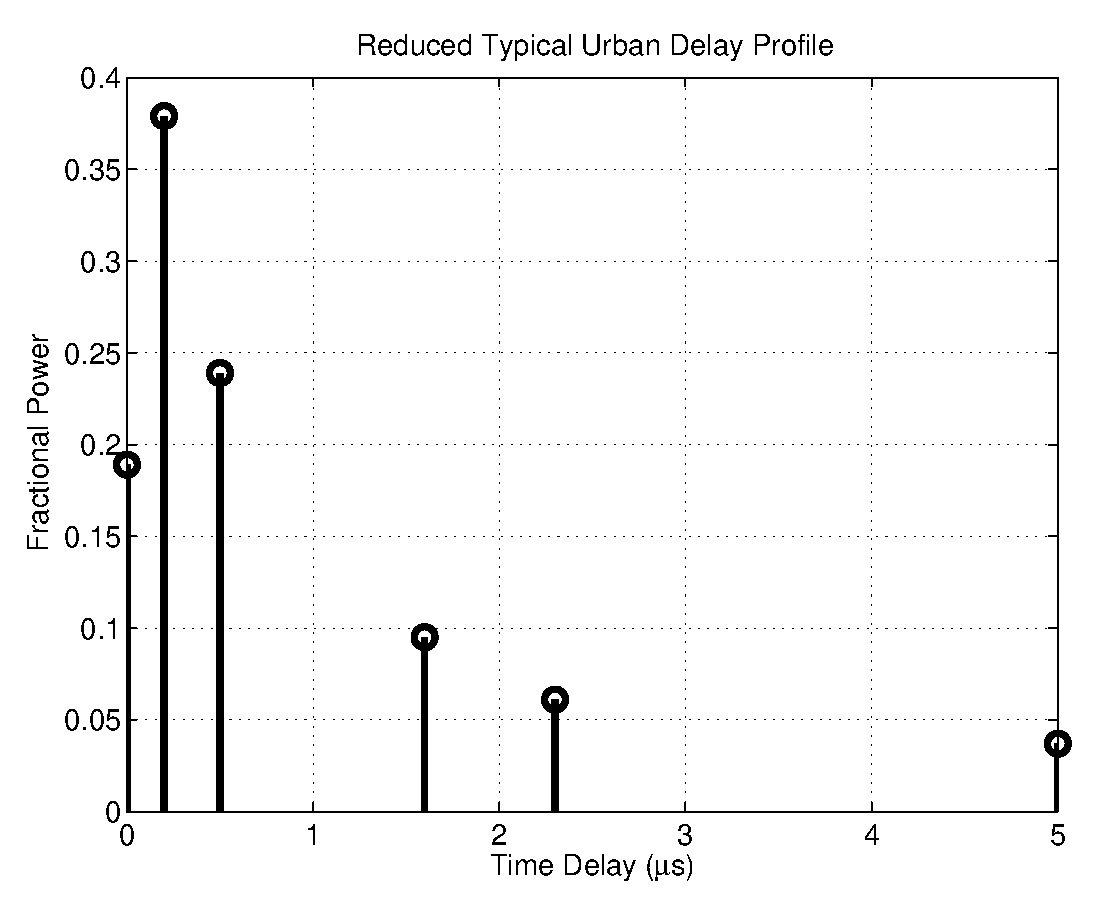
\includegraphics[width=.6\linewidth]{power_delay_profile.eps}
\caption{The power delay profile of the reduced typical urban (TU).}\label{fig:delay_profile}
\end{figure}

The approach we use to implement the channel with given Doppler Spectrum is via the sum-of-sinusoids method. That is based on 
\begin{equation}
g(t)=\sum^N_{n=1}\alpha_n(t)e^{-j\phi_n(t) }, 
\end{equation}
where $\phi_n(t)=2\pi{(f_c+f_{D,n}(t))\tau_n(t)-f_{D,n}(t)t}$ and $N$ is the number of the incoming signals. (1) can be approximated as
\begin{equation}
\begin{aligned}
g(t)=&\sqrt{2}\Big([2\sum^M_{n=1}A_{k,n}\cos\beta_n\cos 2\pi f_n t+\sqrt{2}\cos\alpha\cos 2\pi f_m t] \\
&+j[2\sum^M_{n=1}A_{k,n}\sin\beta_n\cos 2\pi f_n t+\sqrt{2}\sin\alpha\cos 2\pi f_mt ]\Big),
\end{aligned}
\end{equation}
and set $M = \frac{1}{2}(\frac{N}{2}-1)$, $f_n = f_m\cos(\theta)$, $\beta_n=\frac{\pi n}{M}$ and $\alpha=0$, where $\theta$ depends on the Doppler spectrum of a tap ,and $A_{k,n}$ is the $k$-th row of Hadamard matrix which is used to decorrelate the fading envelopes. Note that $ \theta =  \frac{2\pi n}{N}$, which is assumed that is isotropic scattering with uniform incoming signals, if the Doppler category is CLASS. Otherwise, $\theta$ is certain angles, which means the received signals are non-isotropic scattering, if the Doppler category is GAUS1 or GAUS2. Based on the method mentioned above, the channel of each tap can be simulated. We can further combine these channels in terms of the power delay profile depicted in Fig. \ref{fig:delay_profile}. Multiply the channel gain to each tap and shift that with given delay, and then sum all taps signal up. We can get the channel output of the six-tap reduced typical urban.

\newpage

\section{Numerical Results}
In this section, we demonstrate the outputs of the channel emulator. The number of the oscillators of the sum-of-sinusoids method is $M=16$, and the carrier frequency is $f_c = 2$ (GHz). In addition, the sampling frequency is $f_s = 1$ (KHz). There is a mobile user moving with velocity $v$ and we simulate the channel outputs with $v=50$ (km/hr) and $v= 90$ (km/hr), respectively, to see the impact the Doppler shift.

The simulation results are organized as follows.
The outputs of the taps are shown in Fig. \ref{fig:strength_scatterings}-\ref{fig:crosscorr} and the autocorrelations of that is shown in Fig. \ref{fig:autocorr_all}. 
The fading distribution is shown in Fig.\ref{fig:fading_distribution}. 
Some time-domain characteristics are shown in Fig.  \ref{fig:strength_time}-\ref{fig:level crossing90}, and some frequency-domain characteristics are shown in Fig. \ref{fig:strength_freq}-\ref{fig:psd_channel}.


More specifically, in Fig. \ref{fig:autocorr_all}, we can see that the channel correlations of GAUS1 and GAUS2 are much higher than that of CLASS due to both of them are non-isotropic and this result can be also observed in Fig. \ref{fig:strength_scatterings}. Moreover, in Fig. \ref{fig:dopplerspectrum}, the spectrums of CLASS, GAUS1 and GAUS2 derived from the emulator output are similar to the theoretical results, where CLASS is an U-shape and GUAS1/2 is a sum of two Gaussian distribution, one's amplitude is much larger than the other one's amplitude. In Fig. \ref{fig:crosscorr}, we can see that the correlations between two different taps are close to zero. In other word, the cross-correlation between the different generated fading envelopes with modification is not significant.



In Fig. \ref{fig:fading_distribution}, we can observe that when the mobile velocity is low, the number of the deep fades is fewer than that in high mobile velocity since the maximum Doppler shift is linear in mobile speed. As a mobile user moves with high speed, the channel condition varies frequently such that it is difficult to estimate the received signals correctly. Thus, the probability of the channel in deep fade is lower when a mobile user is in low speed. For example, in Fig. \ref{fig:strength_time}, it is clear to see that there are four fades which are lower than $-40$ dB when $v = 90$ (km/hr), whereas there is only one fade lower than $-40$ dB when $v = 50$ (km/hr).



In Fig. \ref{fig:level crossing50}, we demonstrate the level crossing rate and average fade duration varying the threshold. We can see that the level crossing rate increases as the threshold varies from $-20$ dB to $-5$ dB in our scenario since there are few deep fades that can cross low envelope level. When the threshold is greater than $0$ dB, the level crossing rate decreases since there are not too many fades with high channel gain. Moreover, the average fade duration increases as the threshold increases since only a few of deep fades which fading duration is very short are across the level threshold that is low. In Fig. \ref{fig:level crossing90}, we can still observe similar results mentioned above when the mobile velocity is $90$ (km/hr). The difference is that the crossing rate as $v= 90$ (km/hr) is higher than that as $v=50$ (km/hr) under the same threshold ($-20$ dB to $10$ dB) because the effect of the Doppler shift is significant  such that there are too many deep fades in high mobile speed.



We implement the autocorrelation in the frequency domain by transferring the time-domain signal into frequency domain. Next, this frequency-domain signal is multiplied by its conjugate signal, and then take the inverse Fourier transform. Eventually, we can get the autocorrelation of the desired signal. We can see the results in Fig. \ref{fig:autocorr_channel_freq} are the same as those in Fig. \ref{fig:autocorr_channel_time}. In other word, the correlation in time domain is equivalent to the multiplication in frequency domain.



The frequency-domain strength profile and the power spectrum density of the six-tap channel are shown in Fig. \ref{fig:strength_freq} and Fig. \ref{fig:psd_channel}, respectively. It can be observed that the most power are distributed within $(0, f_m)$, where $f_m$ is the maximum Doppler frequency. We can also find the value of $f_m$ according to these two figures. For example, in Fig.  \ref{fig:strength_freq}(a) or Fig.\ref{fig:psd_channel}(a), we can see that the maximum Doppler frequency is about $92$ (Hz). The theoretical value of that is $\frac{v\times f_c}{c} = \frac{50\times1000/3600}{2\times10^9\times 3\times10^8}\approx 92.59$ (Hz). Both values are very close.



%\subsection{Doppler Spectrums}
\begin{figure}[t]
%\graphicspath{fig/}
\centering
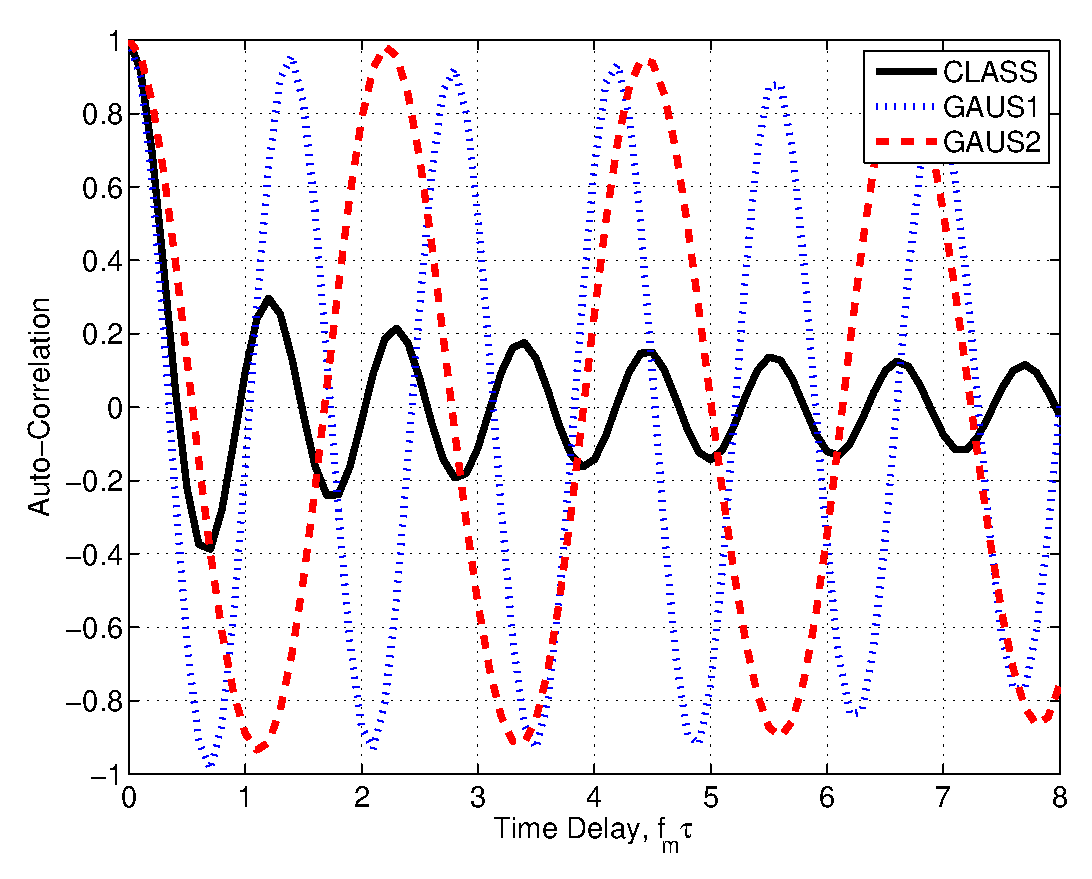
\includegraphics[width=.6\linewidth]{autocorr_compareall_v50.eps}
\caption{Auto-correlation of different Doppler patterns at $v = 50$ (km/hr).}\label{fig:autocorr_all}
\end{figure}

\begin{figure}[t]
%\graphicspath{fig/}
\centering
\subfigure[CLASS]{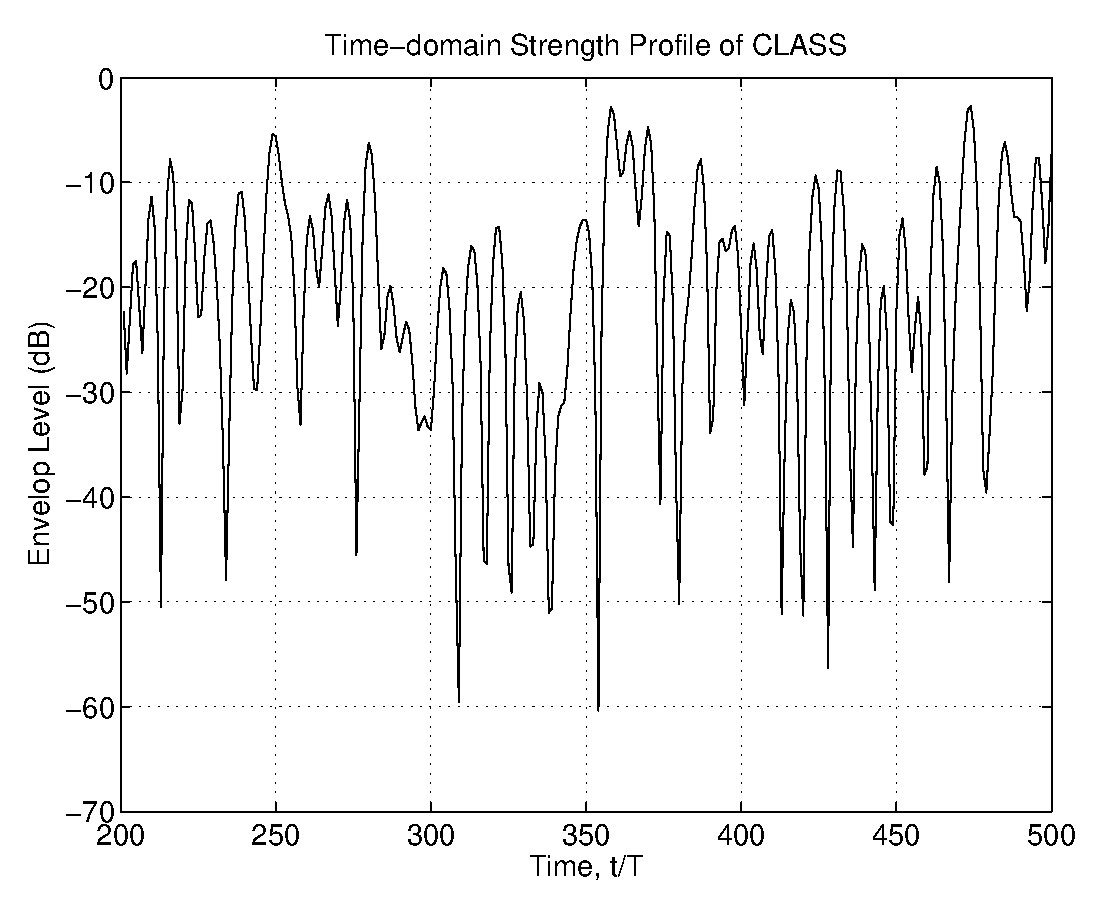
\includegraphics[width=.5\linewidth]{strength_time_class_v50}}
\subfigure[GAUS1]{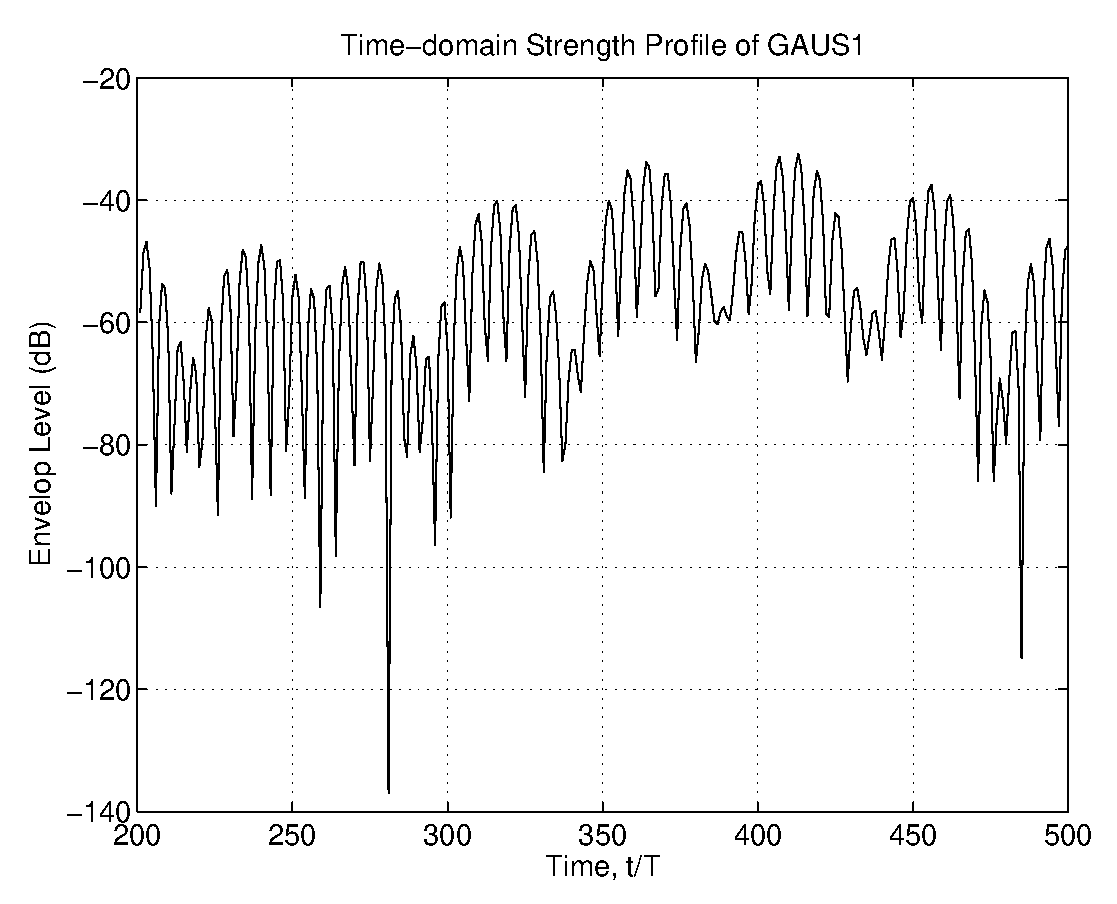
\includegraphics[width=.5\linewidth]{strength_time_gaus1_v50}}
\subfigure[GAUS2]{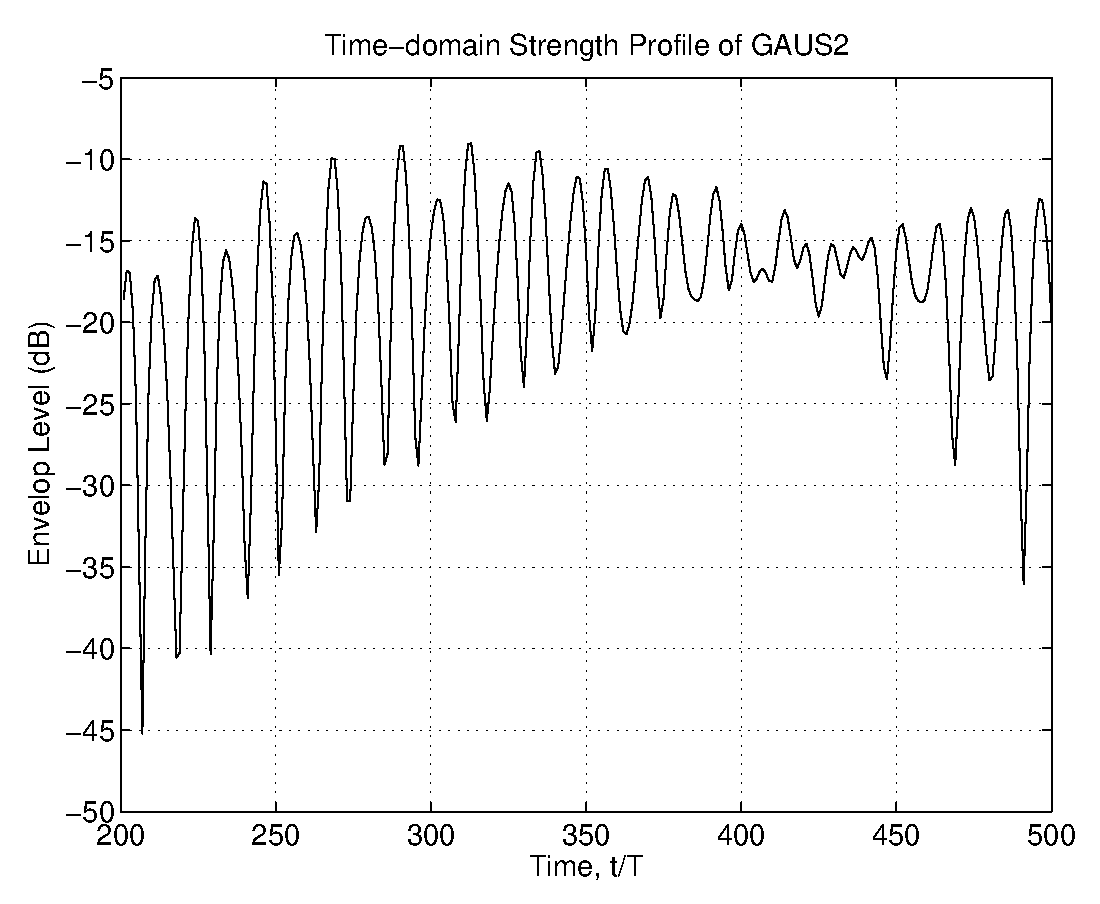
\includegraphics[width=.5\linewidth]{strength_time_gaus2_v50}}
\caption{The time-domain strength of CLASS, GAUS1 and GAUS2 at $v=50$ (km/hr).}\label{fig:strength_scatterings}
\end{figure}



\begin{figure}[t]
%\graphicspath{fig/}
\centering
\subfigure[Classical Doppler spectrum]{\includegraphics[width=.5\linewidth]{psd_class_v50.eps}}
\subfigure[Gaussian $1$ Doppler spectrum]{\includegraphics[width=.5\linewidth]{psd_gaus1_v50.eps}}
\subfigure[Gaussian $2$ Doppler spectrum]{\includegraphics[width=.5\linewidth]{psd_gaus2_v50.eps}}
\caption{The Doppler spectrums of COST 207 at $v=50$ (km/hr).}\label{fig:dopplerspectrum}
\end{figure}




\begin{figure}[t]
%\graphicspath{fig/}
\centering
\includegraphics[width=.6\linewidth]{crosscorr_v50.eps}
\caption{Cross-correlation between two different taps at $v = 50$ (km/hr)}\label{fig:crosscorr}
\end{figure}

%\newpage
%\subsection{Time-Domain Characteristics}

\begin{figure}[t]
%\graphicspath{fig/}
\centering
\subfigure[Mobile velocity $= 50$ (km/hr)]{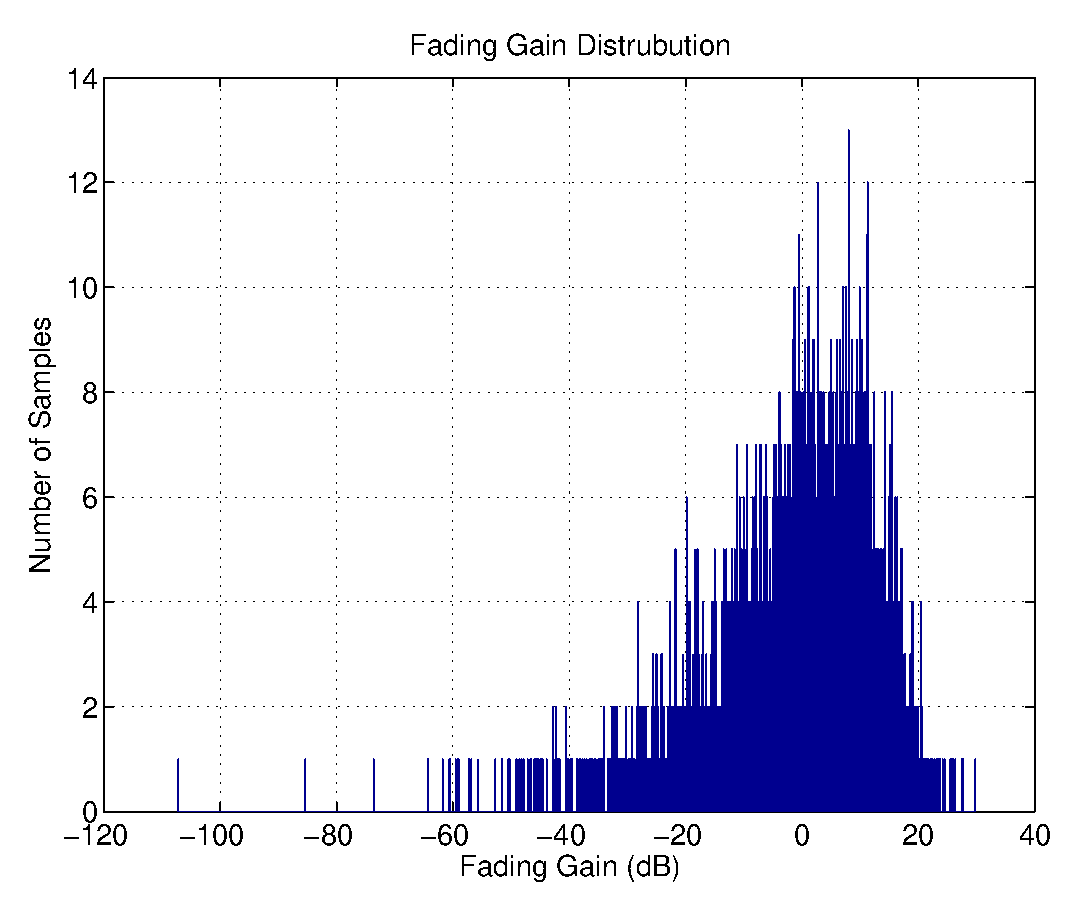
\includegraphics[width=.45\linewidth]{fading_gain_distribution_v50.eps}}
\subfigure[Mobile velocity $= 90$ (km/hr)]{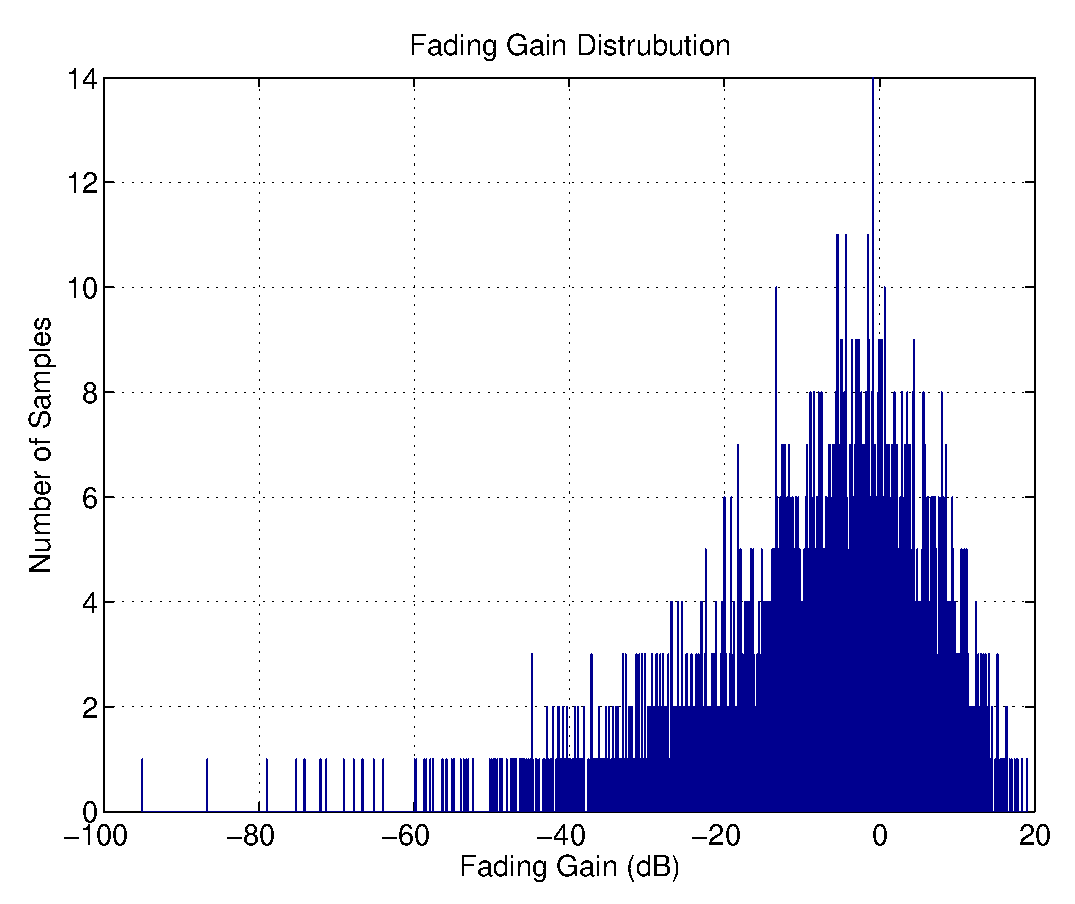
\includegraphics[width=.45\linewidth]{fading_gain_distribution_v90.eps}}
\caption{Fading Distribution under different mobile velocity.}\label{fig:fading_distribution}
\end{figure}

\begin{figure}[t!]
%\graphicspath{fig/}
\centering
\subfigure[Mobile velocity $= 50$ (km/hr).]{\includegraphics[width=.45\linewidth]{strength_time_v50.eps}}
\subfigure[Mobile velocity $= 90$ (km/hr).]{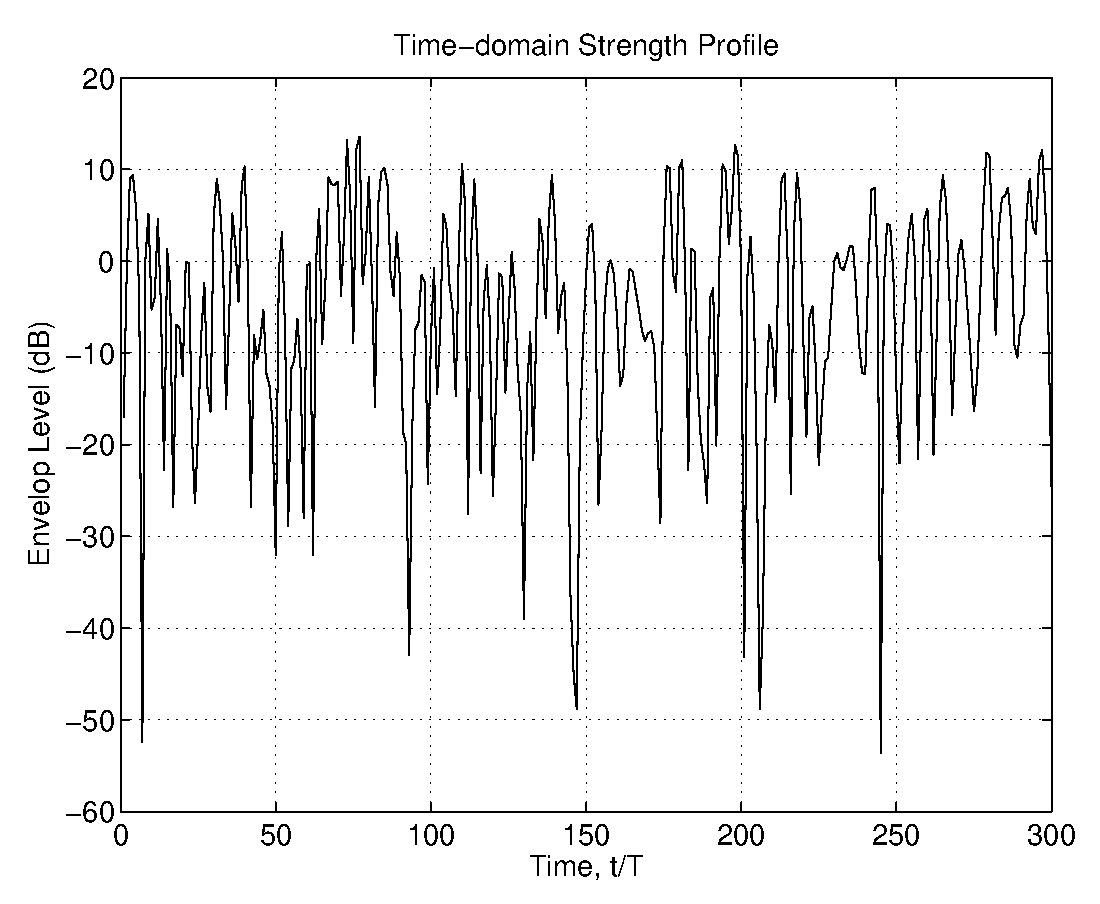
\includegraphics[width=.45\linewidth]{strength_time_v90.eps}}
\caption{Time-domain strength profile under different mobile velocity.}\label{fig:strength_time}
\end{figure}

\begin{figure}[t!]
%\graphicspath{fig/}
\centering
\subfigure[Mobile velocity $= 50$ (km/hr).]{\includegraphics[width=.45\linewidth]{autocorr_channel_time_v50.eps}}
\subfigure[Mobile velocity $= 90$ (km/hr).]{\includegraphics[width=.45\linewidth]{autocorr_channel_time_v90.eps}}
\caption{Auto-correlation (time-domain) of the six-tap channel under different mobile velocity.}\label{fig:autocorr_channel_time}
\end{figure}

\begin{figure}[t!]
%\graphicspath{fig/}
\centering
\subfigure[Level crossing rate]{\includegraphics[width=.45\linewidth]{crossingrate_v50.eps}}
\subfigure[Average fade duration]{\includegraphics[width=.45\linewidth]{avgfade_duration_v50.eps}}
\caption{Level crossing rate and average fade duration under different threshold as $v = 50$ (km/hr).}\label{fig:level crossing50}
\end{figure}

\begin{figure}[t!]
%\graphicspath{fig/}
\centering
\subfigure[Level crossing rate]{\includegraphics[width=.45\linewidth]{crossingrate_v90.eps}}
\subfigure[Average fade duration]{\includegraphics[width=.45\linewidth]{avgfade_duration_v90.eps}}
\caption{Level crossing rate and average fade duration under different threshold as $v = 90$ (km/hr).}\label{fig:level crossing90}
\end{figure}

%\newpage
%\subsection{Frequency-Domain Characteristics}

\begin{figure}[t]
%\graphicspath{fig/}
\centering
\subfigure[Mobile velocity $= 50$ (km/hr).]{\includegraphics[width=.45\linewidth]{strength_freq_v50.eps}}
\subfigure[Mobile velocity $= 90$ (km/hr).]{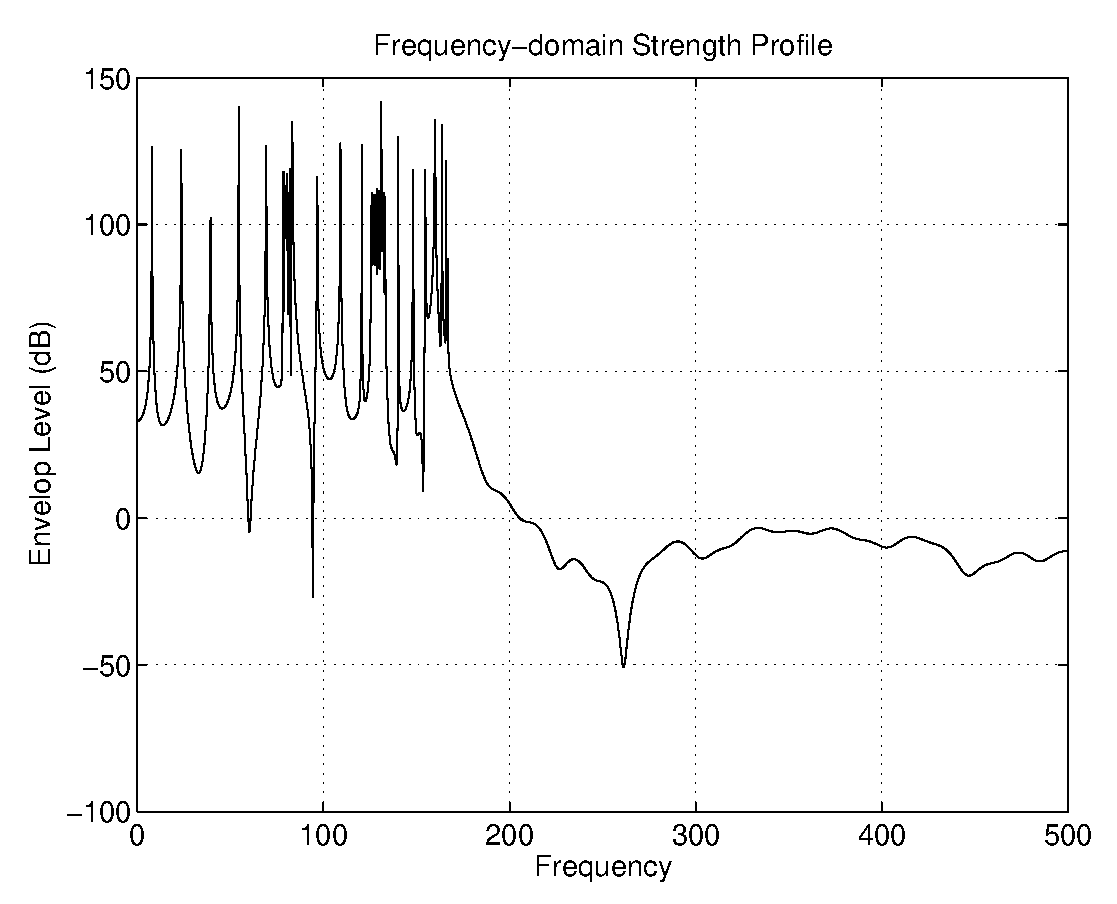
\includegraphics[width=.45\linewidth]{strength_freq_v90.eps}}
\caption{Frequency-domain strength profile under different mobile velocity.}\label{fig:strength_freq}
\end{figure}

\begin{figure}[t]
%\graphicspath{fig/}
\centering
\subfigure[Mobile velocity $= 50$ (km/hr).]{\includegraphics[width=.45\linewidth]{autocorr_channel_freq_v50.eps}}
\subfigure[Mobile velocity $= 90$ (km/hr).]{\includegraphics[width=.45\linewidth]{autocorr_channel_freq_v90.eps}}
\caption{Auto-correlation (frequency-domain) of the six-tap channel under different mobile velocity.}\label{fig:autocorr_channel_freq}
\end{figure}

\begin{figure}[t]
%\graphicspath{fig/}
\centering
\subfigure[Mobile velocity $= 50$ (km/hr).]{\includegraphics[width=.45\linewidth]{psd_channel_v50.eps}}
\subfigure[Mobile velocity $= 90$ (km/hr).]{\includegraphics[width=.45\linewidth]{psd_channel_v90.eps}}
\caption{Power spectrum density of the six-tap channel under different mobile velocity}\label{fig:psd_channel}
\end{figure}









\end{document}